% Created 2026-07-09 jue 23:47
% Intended LaTeX compiler: pdflatex
\documentclass{article}
\usepackage[utf8]{inputenc}
\usepackage[T1]{fontenc}
\usepackage{graphicx}
\usepackage{longtable}
\usepackage{wrapfig}
\usepackage{rotating}
\usepackage[normalem]{ulem}
\usepackage{amsmath}
\usepackage{amssymb}
\usepackage{capt-of}
\usepackage{hyperref}

\usepackage{fancyhdr}
\usepackage[top=25mm, left=25mm, right=25mm]{geometry}
\usepackage{longtable}
\fancyhead[R]{}
\setlength\headheight{43.0pt}
\usepackage[T1]{fontenc}
\usepackage[utf8]{inputenc}
\usepackage[spanish, ]{babel}
\usepackage[backend=biber]{biblatex}

\author{Juan Auz, Lanchimba Danny, Palomeque Matías, Quillupangui Ana María}
\date{2026-07-09}
\title{Booteo de Sistema Operativo Linux}
\hypersetup{
 pdfauthor={Juan Auz, Lanchimba Danny, Palomeque Matías, Quillupangui Ana María},
 pdftitle={Booteo de Sistema Operativo Linux},
 pdfkeywords={},
 pdfsubject={},
 pdfcreator={Emacs 27.1 (Org mode 9.7.5)}, 
 pdflang={Español}}
\begin{document}

\maketitle
\fancyhead[C]{\includegraphics[scale=0.05]{images/logoEPN.jpg}\\
ESCUELA POLITÉCNICA NACIONAL\\FACULTAD DE INGENIERÍA DE SISTEMAS\\
ARQUITECTURA DE COMPUTADORES}
\thispagestyle{fancy}
\section{Objetivos}
\label{sec:org15b09d8}

\begin{itemize}
\item Aprender a  bootear un sistema operativo Linux

\item Aprender sobre la secuencia de arranque de un computador como la
BIOS y la UEFI
\end{itemize}
\section{Instrucciones}
\label{sec:orgab040be}
\begin{enumerate}
\item Siga el tutorial para la creación de un booteable de Ubuntu como se
indica en la unidad 9 en el archivo Arranque Ubuntu\footnote{Dependiendo de las características de su computador debe
verificar si al crear el medio booteable para Ubuntu, su sistema
reconoce o acepta para el \emph{Target System}}.

\item Realice un respaldo del código de \emph{BitLocker} utilizando un command
prompt de Windows con permisos de administrador\footnote{Si no respalda el código, no podrá arrancar el disco luego de
reiniciar. Más información en: \href{https://www.partitionwizard.com/disk-recovery/bitlocker-recovery-key-bypass.html }{https://www.partitionwizard.com/disk-recovery/bitlocker-recovery-key-bypass.html}}:

\begin{verbatim}
    manage-bde-protectors C:-get
\end{verbatim}

\item Utilizando su computador o el del laboratorio, siga los pasos
indicados para obtener el booteo desde el USB con el Sistema
Operativo de Ubuntu

\item Realice el boot de Ubuntu desde la memoria USB externa y
seleccione la opción de \emph{Probar Sistema Operativo}.
\item Una vez ingresado active un terminal de Ubuntu: \texttt{Ctrl+ALT+T} y
obtenga las características del computador mediante la ejecución de
los comandos: \texttt{lscpu}, \texttt{lsb\_release -a} y \texttt{lspci}. Obtenga capturas
de la ejecución de los comandos. Luego abra este archivo en WSL y
ejecute los comandos desde los bloques shell. Para insertar un
bloque puede usar la combinación \texttt{C-c C-,}, escoja la opción \texttt{src}
e indique que es del tipo shell.
\end{enumerate}
\section{Desarrollo Emacs}
\label{sec:org21331f9}
Se sugiere utilizar la opción \texttt{:fontsize
scriptsize} para dar formato a la ejecución del comando. Por ejemplo,
considere:

\begin{verbatim}
whoami
\end{verbatim}

\phantomsection
\label{org98399c1}
\begin{verbatim}
juand
\end{verbatim}
\subsection{Comando \texttt{lsb\_release}}
\label{sec:orgfe62b15}
\begin{verbatim}
    lsb_release -a
\end{verbatim}

\phantomsection
\label{org49d32d1}
\begin{verbatim}
LSB Version:	n/a
Distributor ID:	Arch
Description:	Arch Linux
Release:	rolling
Codename:	n/a
\end{verbatim}
\subsection{Comando \texttt{lspci}}
\label{sec:org2abf461}
\begin{verbatim}
    lspci
\end{verbatim}

\phantomsection
\label{org6dd9d7d}
\begin{verbatim}
   00:00.0 Host bridge: Advanced Micro Devices, Inc. [AMD] Family 15h (Models 60h-6fh) Processor Root Complex
   00:00.2 IOMMU: Advanced Micro Devices, Inc. [AMD] Family 15h (Models 60h-6fh) I/O Memory Management Unit
   00:01.0 VGA compatible controller: Advanced Micro Devices, Inc. [AMD/ATI] Stoney [Radeon R2/R3/R4/R5 Graphics] (rev ea)
   00:01.1 Audio device: Advanced Micro Devices, Inc. [AMD/ATI] Stoney HDMI/DP Audio Controller
   00:02.0 Host bridge: Advanced Micro Devices, Inc. [AMD] Family 15h (Models 60h-6fh) Host Bridge
   00:02.1 PCI bridge: Advanced Micro Devices, Inc. [AMD] Family 15h (Models 60h-6fh) Processor Root Port
   00:02.2 PCI bridge: Advanced Micro Devices, Inc. [AMD] Family 15h (Models 60h-6fh) Processor Root Port
   00:02.3 PCI bridge: Advanced Micro Devices, Inc. [AMD] Family 15h (Models 60h-6fh) Processor Root Port
   00:03.0 Host bridge: Advanced Micro Devices, Inc. [AMD] Family 15h (Models 60h-6fh) Host Bridge
   00:08.0 Encryption controller: Advanced Micro Devices, Inc. [AMD] Carrizo Platform Security Processor
   00:09.0 Host bridge: Advanced Micro Devices, Inc. [AMD] Carrizo Audio Dummy Host Bridge
   00:09.2 Audio device: Advanced Micro Devices, Inc. [AMD] Family 15h (Models 60h-6fh) Audio Controller
   00:10.0 USB controller: Advanced Micro Devices, Inc. [AMD] FCH USB XHCI Controller (rev 20)
   00:11.0 SATA controller: Advanced Micro Devices, Inc. [AMD] FCH SATA Controller [AHCI mode] (rev 4b)
   00:12.0 USB controller: Advanced Micro Devices, Inc. [AMD] FCH USB EHCI Controller (rev 49)
   00:14.0 SMBus: Advanced Micro Devices, Inc. [AMD] FCH SMBus Controller (rev 4b)
   00:14.3 ISA bridge: Advanced Micro Devices, Inc. [AMD] FCH LPC Bridge (rev 11)
   00:18.0 Host bridge: Advanced Micro Devices, Inc. [AMD] Stoney HT Configuration
   00:18.1 Host bridge: Advanced Micro Devices, Inc. [AMD] Stoney Address Maps
   00:18.2 Host bridge: Advanced Micro Devices, Inc. [AMD] Stoney DRAM Configuration
   00:18.3 Host bridge: Advanced Micro Devices, Inc. [AMD] Stoney Miscellaneous Configuration
   00:18.4 Host bridge: Advanced Micro Devices, Inc. [AMD] Stoney PM Configuration
   00:18.5 Host bridge: Advanced Micro Devices, Inc. [AMD] Stoney NB Performance Monitor
   02:00.0 Ethernet controller: Realtek Semiconductor Co., Ltd. RTL8111/8168/8211/8411 PCI Express Gigabit Ethernet Controller (rev 15)
   03:00.0 Network controller: Realtek Semiconductor Co., Ltd. RTL8723DE 802.11b/g/n PCIe Adapter
\end{verbatim}
\subsection{Comando \texttt{lscpu}}
\label{sec:org538b9d0}
\begin{verbatim}
 lscpu
\end{verbatim}

\phantomsection
\label{orgd47c029}
\begin{verbatim}
   Arquitectura:                             x86_64
   modo(s) de operación de las CPUs:         32-bit, 64-bit
   Tamaños de las direcciones:               48 bits physical, 48 bits virtual
   Orden de los bytes:                       Little Endian
   CPU(s):                                   2
   Lista de la(s) CPU(s) en línea:           0,1
   ID de fabricante:                         AuthenticAMD
   Nombre del modelo:                        AMD A6-9225 RADEON R4, 5 COMPUTE CORES 2C+3G
   Familia de CPU:                           21
   Modelo:                                   112
   Hilo(s) de procesamiento por núcleo:      1
   Núcleo(s) por «socket»:                   2
   «Socket(s)»:                              1
   Revisión:                                 0
   Microcode version:                        0x6006705
   Aumento de frecuencia:                    activada
   CPU(s) factor de escala MHz:              100%
   CPU MHz máx.:                             2600,0000
   CPU MHz mín.:                             1300,0000
   BogoMIPS:                                 5190,11
   Indicadores:                              fpu vme de pse tsc msr pae mce cx8 apic sep mtrr pge mca cmov pat pse36 clflush mmx fxsr sse sse2 ht syscall nx mmxext fxsr_opt pdpe1gb rdtscp lm constant_tsc rep_good acc_power nopl nonstop_tsc cpuid extd_apicid aperfmperf pni pclmulqdq monitor ssse3 fma cx16 sse4_1 sse4_2 movbe popcnt aes xsave avx f16c lahf_lm cmp_legacy svm extapic cr8_legacy abm sse4a misalignsse 3dnowprefetch osvw ibs xop skinit wdt lwp fma4 tce nodeid_msr tbm perfctr_core perfctr_nb bpext ptsc mwaitx cpb hw_pstate ssbd ibpb vmmcall fsgsbase bmi1 avx2 smep bmi2 xsaveopt arat npt lbrv svm_lock nrip_save tsc_scale vmcb_clean flushbyasid decodeassists pausefilter pfthreshold avic v_vmsave_vmload vgif overflow_recov
   Virtualización:                           AMD-V
   Caché L1d:                                64 KiB (2 instancias)
   Caché L1i:                                192 KiB (2 instancias)
   Caché L2:                                 2 MiB (2 instancias)
   Modo(s) NUMA:                             1
   CPU(s) del nodo NUMA 0:                   0,1
   Vulnerabilidad Gather data sampling:      Not affected
   Vulnerabilidad Ghostwrite:                Not affected
   Vulnerabilidad Indirect target selection: Not affected
   Vulnerabilidad Itlb multihit:             Not affected
   Vulnerabilidad L1tf:                      Not affected
   Vulnerabilidad Mds:                       Not affected
   Vulnerabilidad Meltdown:                  Not affected
   Vulnerabilidad Mmio stale data:           Not affected
   Vulnerabilidad Old microcode:             Not affected
   Vulnerabilidad Reg file data sampling:    Not affected
   Vulnerabilidad Retbleed:                  Mitigation; untrained return thunk; SMT disabled
   Vulnerabilidad Spec rstack overflow:      Not affected
   Vulnerabilidad Spec store bypass:         Mitigation; Speculative Store Bypass disabled via prctl
   Vulnerabilidad Spectre v1:                Mitigation; usercopy/swapgs barriers and __user pointer sanitization
   Vulnerabilidad Spectre v2:                Mitigation; Retpolines; IBPB conditional; STIBP disabled; RSB filling; PBRSB-eIBRS Not affected; BHI Not affected
   Vulnerabilidad Srbds:                     Not affected
   Vulnerabilidad Tsa:                       Not affected
   Vulnerabilidad Tsx async abort:           Not affected
   Vulnerabilidad Vmscape:                   Not affected
\end{verbatim}
\section{Desarrollo Capturas}
\label{sec:org02d967b}
Coloque las capturas de los resultados obtenidos en los
terminales. Para esto recuerde utilizar dobles corchetes y escribir el
\emph{path} hacia la imagen. Pruebe a utilizar YASnipet para generar el
siguiente código para descripción de la figura. Para esto puede
escriba \texttt{fig\_} seguido de la combinación de teclas \texttt{C-TAB}, finalmente
coloque la dirección de la imagen.

\begin{figure}[htbp]
\centering
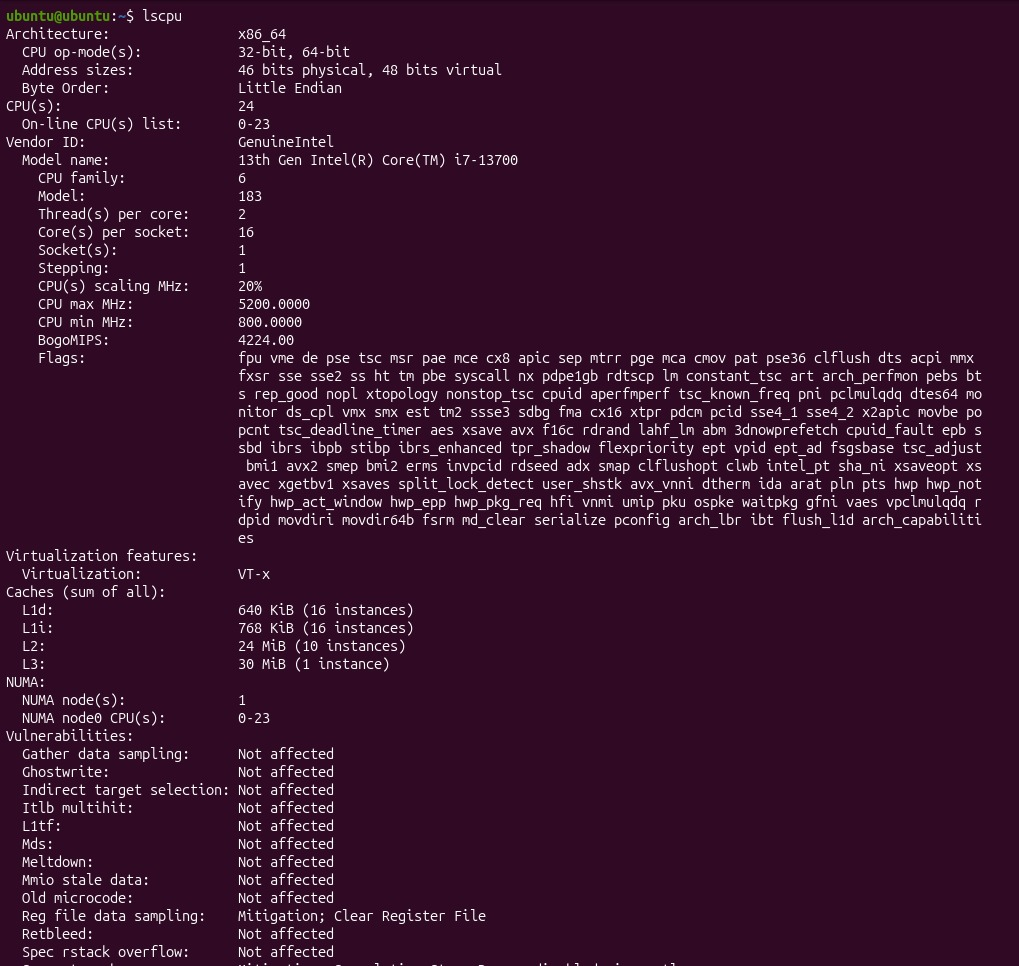
\includegraphics[width=.9\linewidth]{images/lscpu1.jpeg}
\caption{\label{fig:org9ef4f45}Resultado del comando lscpu1}
\end{figure}

\begin{figure}[htbp]
\centering
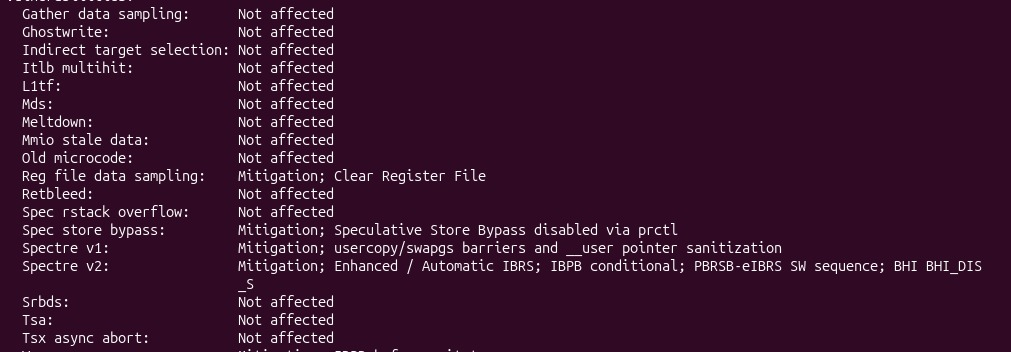
\includegraphics[width=.9\linewidth]{images/lscpu2.jpeg}
\caption{\label{fig:org80b28b2}Resultado del comando lscpu2}
\end{figure}

\begin{figure}[htbp]
\centering
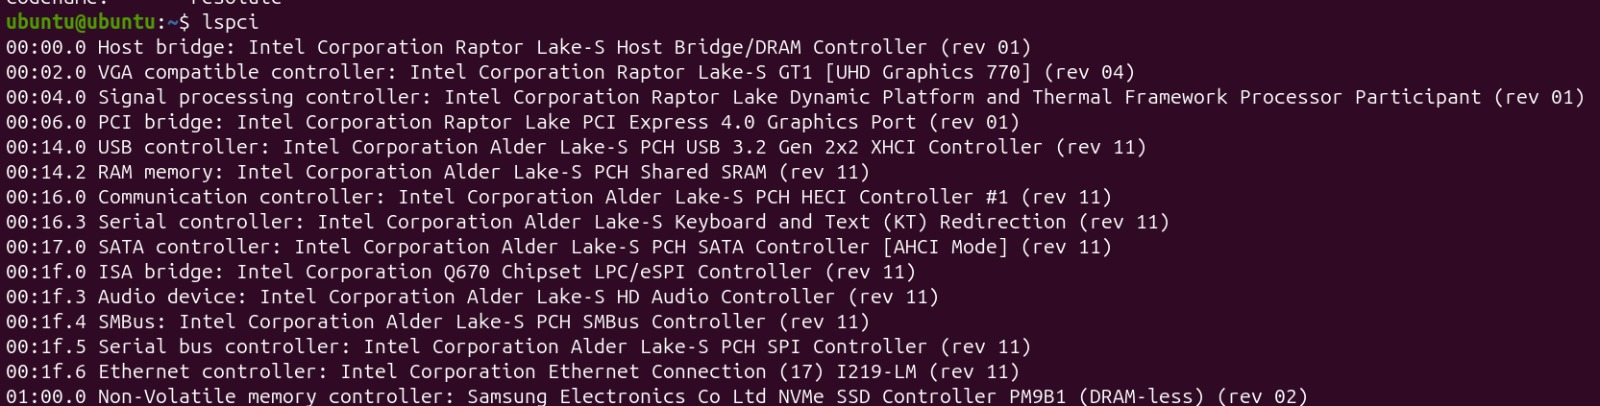
\includegraphics[width=.9\linewidth]{images/lscpi.jpeg}
\caption{\label{fig:org99ddcfd}Resultado de lscpi}
\end{figure}

\begin{figure}[htbp]
\centering
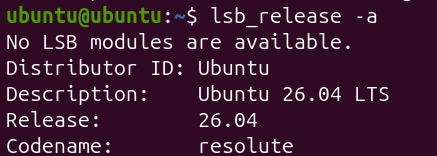
\includegraphics[width=.9\linewidth]{images/lsb_release.jpeg}
\caption{\label{fig:orgd3502f2}Resultado de lsb\textsubscript{release}}
\end{figure}

\begin{figure}[htbp]
\centering
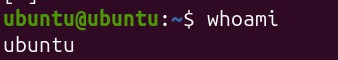
\includegraphics[width=.9\linewidth]{images/whoami.jpeg}
\caption{\label{fig:org2133c70}Resultado de whoami}
\end{figure}
\section{Consulta}
\label{sec:org7e4aaef}
Describa que hacen y para qué sirven los comandos utilizados en la práctica

\begin{description}
\item[{lscpu}] \texttt{lscpu} Muestra la información detallada acerca la arquitectura y el
procesador del sistema. Se lo utiliza para conocer las
características del procesador, como:
\begin{itemize}
\item Arquitectura (34 o 64 bits).
\item Modelo y fabricante de la CPU.
\item Número de núcelos e hilos.
\item Frecuencia delprocesador.
\item Memoria caché.
\item Teconologías soportadas (virtualización, entre otras).
\end{itemize}

\item[{lsb$\backslash$\textsubscript{release} -a}] \texttt{lsb\_release -a} Muestra la información acerca de la distribución de
linux instalada. Nos permite identificar la versión y los datos de
la distribución del sistema operativo, incluyendo:
\begin{itemize}
\item Nombre de la distribución.
\item Descripción acerca de la versión que posee.
\item Descripción del sistema.
\end{itemize}

\item[{lspci}] \texttt{lspci} Lista todos los dispositivos al bus PCI del equipo. Sirve
para identificar el hardware conectado al sistema, por ejemplo:
\begin{itemize}
\item Tarjeta Gráfica.
\item Tarjeta de red.
\item Controladores SATA o NVMe.
\item Dispositivos de audio.
\item Controladores USB.
\end{itemize}
\end{description}
\end{document}
